\documentclass[aps,showpacs,twocolumn,floatfix,prx,superscriptaddress]{revtex4-1}
\usepackage{graphicx}
\usepackage{amsfonts}
\usepackage{amsmath}
\usepackage{amssymb}
\usepackage{upgreek}
\usepackage[usenames,dvipsnames]{color}

%\bibliographystyle{apsrev}


\begin{document}

\title{Yet another mapping to ASEP --- 1D polymer dynamics}

\author{Wenwen Huang}
\author{Yen Ting Lin}
\author{Daniela Fr\"{o}mberg}
\author{Jaeoh Shin}
\author{Frank J\"{u}licher}
\author{Vasily Zaburdaev}
\affiliation{Max Planck Institute for the Physics of Complex Systems, N\"{o}thnitzer Str. 38, D-01187 Dresden, Germany}

\begin{abstract}
{}
\end{abstract}
\maketitle


\section{Introduction}
Many biological processes can be described by idealized physical models and
quantitatively studied through the law of physics and methods of mathematics.  A
good example is the movement of DNA. Polymer models, constructed by bead and rod
or spring, are often utilized to describe DNA\cite{}.  In our study of
chromosome alignment in meiotic fission yeast, a freely jointed bead rod ring
model is adopted\cite{}. Chromosomes during the stage of nuclear oscillation are
translated to pinned polymer loop in an external field\cite{}. To further
understand the physics of such pinned polymer loop model, here we formulate the
problem in 1D, i.e. rods orientate either right or left. Amazingly, we found
this simple model can maps to a 1D particle hopping problem, well known as
asymmetric simple exclusion process (ASEP)\cite{}. On the other hand, ASEP
itself is a well studied paradigmatic model in non-equilibrium statistics with
thousands of applications\cite{}. It turns out many real problems can be mapped
to ASEP.  For instance, ASEP is frequently used to model the traffic
transportation\cite{}.  Another example is ref. \cite{}, MacDonald et al. shown
their pioneering work to use ASEP quantitatively modelling kinetic of
biopolymerization. Also in ref.  \cite{}, the reptation movement of polymer in
crowded environment is again mapped to ASEP model.  In this paper, we will add
one more class of problems which can be exactly mapped to ASEP --- 1D polymer
dynamics. Notice the polymer here is in general polymers in dilute solution rather
than the reptating polymer in crowded environment.  

In this paper, we will show how to map from a pinned polymer model describing
chromosomes to an ASEP particle hopping process. The equivalence between these
two models means that methods used to solve one problem can also be mapped to
solve the other. As ASEP is a well studied exactly solvable system, we
demonstrate that the analytical results can also be translated to the problem of
polymer dynamics. In addition, we show that the famous Fermi-Dirac statistics
serves as an asymptotic approximation of statistics for rod orientation as well
as the density profile of particles. All results shown here are verified by
numerical simulations. To further demonstrate the power of this mapping, we
study the relaxation of polymer represented by the mapped particle hopping
process and compared with the Rouse theory and Brownian Dynamics (BD)
simulations.  Interestingly, we found the relaxation time of gyration radius
varies non-monotonically with the external force, which is consistent with 3D
theory and simulations.

The next section we will describe how to build the mapping from polymer and
particle and demonstrate how to draw the useful analytical results through the
mapping. In section III, the mapping is extended to non-equilibrium aspects to
demonstrate its power of prediction. Comparisons of Rouse theory and BD
simulations are discussed in detail. Finally, conclusion remarks and outlooks
are list in section IV. 


\section{Mapping from polymer to particle}
In our study of chromosome movements, we use a bead-and-rod model to model the
chromosomes. Here, we reformulate the model in 1D instead of 3D. The 1D model
is extremely simple but still capture the key properties such as the ability to
measure the  alignment of beads along the external force field.  The exciting
thing is we have a peculiar mapping from 1D polymer to particle on lattice sites
as shown below.  

The chromosome consists of $N$ beads freely jointed by $N$ rods forming
a loop; the rod length is chosen to be the Kuhn length $a$ of the chromosome.
The position of the $i^{\rm th}$ bead is denote by $x_i$, and without lost of
generality, the spindle pole body which is pinned after transforming to the
co-moving frame, is defined to be the $0^{\rm th}$ bead. An constant external
force $F$ is applied on every bead after frame transform with direction defined
to be positive along $x$ without loss of generality. The looping topology of
the polymer suggests $x_0=x_N$.  We do not consider the volume exclusion in the
model of polymer. Define the direction of the $i^{\rm th}$ rod to be
$e_i:=x_{i+1} - x_{i}$.  In a one-dimensional setting, $x_i = i a$ where $i \in
\mathbb{Z}$, and $e_i=\pm a$ for $i=0, 1, \ldots, N-1$. The internal energy of
the polymer reads
\begin{align*}
    E  & = -\sum_{i=1}^{N-1} {Fx_i} = -Fa\sum_{i=1}^{N-1} i  \nonumber \\
       & = - Fa \sum_{i=1}^{N-1} \sum_{j=0}^{i-1} \left(2 Z_j - 1\right),
\end{align*}
here $Z_j := \left(e_j/a+1\right)/2$ is a changed variable. By exchanging the
order of the double summation and utilizing the looping condition 
\begin{equation}
    \label{eq:looping}
    \sum_{j=0}^{N-1} e_j = 0,
\end{equation}
we arrive at 
\begin{equation}
    \label{eq:energy}
    E = E_0 + \Delta E \sum_{j=0}^{N-1} j Z_j
\end{equation}
where $E_0= - N(N-1) \Delta E /2$ and $\Delta E = 2Fa$. 

By observing the energy \eqref{eq:energy}, we immediately recognise that the
system has a Hamiltonian similar to a system with $N/2$ Fermions in an $N$
equally distributed energy levels $0, \Delta E, \ldots, (N-1) \Delta E$, and
$Z_j$ can be interpreted as a binary variable which characterizes whether the
energy level $j$ is occupied ($=1$ if it is occupied, and $=0$ otherwise). 
This is actually the inspiration for us to build the mapping from polymer to
particles. 


% Clearly when the lowest energy corresponds to $Z_j =1$ $\forall j < N/2$ and $Z_j=0$ otherwise. When the system is in contact with an external thermal bath with temperature $T$, it is possible to be in any configuration. The equilibrium Gibbs measure indicates that the probability of the system in a configuration $\l\{Z_j\r\}_{j=0}^{N-1}$ is
% \eq{
% \pr{\l\{Z_j\r\}_{j=0}^{N-1}} \propto \exp \l[-\frac{E_0 + \Delta E \sum_{j=0}^{N-1} j Z_j}{k_B T}\r]
% }{eq:gibbs}
% where $k_B$ is the Boltzmann factor. 
%
% The periodic condition \eqref{eq:periodic} implies a hard constraint of the total number of the Fermions $\sum_{j=0}^{n-1} Z_j = N/2$. This corresponds to a picture of \emph{canonical ensemble} \cite{huang1987statistical}: the system does not exchange particles with its environment. While formally the equilibrium distribution is solved by \eqref{eq:gibbs}, we remark the difficulty of obtaining the analytic solution due to the degeneracy of the system, i.e., some (total) energy levels contain multiple microscopic states. In the next section \ref{sec:partition}, we will illustrate the possibility of obtaining an exact solution using number theory. 
%
% An alternative approach is to first release the fixed-number constraint, and use the \emph{grand canonical ensemble} which allows exchange of particles with external reservoir \cite{huang1987statistical}, derive the probability distribution of the microscopic states to construct an random walk model, and then finally use the to re-enforce the fixed-number constraint \cite{lin2015pulled}. Below we outline the analysis and the results of this approach. In this one-dimensional case,   after releasing the fixed-number constraint, the probability distribution of $Z_j$ can be derived \cite{huang1987statistical} to be a Fermi--Dirac distribution
% \subeq{
% \pr{Z_j = 1} ={}& \l\{1+\exp\l[\frac{ \Delta E \l(j - \mu \r) }{k_B T}\r]\r\}^{-1}, \\
% \pr{Z_j = 0} ={}& 1- \pr{Z_j = 1},
% }{eq:discrete_prob}
% with a chemical potential $\mu = (N-1)/2$ obtained from a symmetry argument. Noting the relation of $Z_j$ and the configuration of the orientation of $j^{\rm th}$ rod $\ve_j = \l(2Z_j -1\r) \Delta l$, the probabilities \eqref{eq:discrete_prob} are used to compute the distribution of $\ve_j$. In this context, the famous Pauli exclusion principle---$Z_j$ can be either 0 or 1---corresponds to an almost trivial statement of each rod: either it points to the right ($Z_j=1$) or to the left ($Z_j=0$). 
%
% We emphasize that only in the picture of grand canonical ensemble, the probability distribution of each rod are mutually independent; with a hard constraint of the particle number, $Z_j$'s are not independently distributed. In fact, the independence is the key for an analytic solutions of the equilibrium properties, such as \eqref{eq:gibbs}, are possible. 
%
% Knowing the probability distribution of the orientation of each rod, a random walk is then built, satisfying the first and the second moments of the individual rods. Specifically, we construct a Gaussian random walk, which satisfies the conditional probability
% \eq{
% \rho\l(\vx_{i+1} \vert \vx_i\r) =\exp\l\{ -\frac{\l[\vx_{i+1}- \vx_i - \l(\Delta l \r) \E{Z_j}\r]^2}{4 \var{Z_j}\Delta l^2}\r\}, 
% }{}
% on a continuum domain $\vx \in \mathbb{R}$. Finally, the ``bridge'' condition in section [XXX] is imposed to re-enforce the fixed-number condition \eqref{eq:periodic}. 
%
% \begin{figure}
% 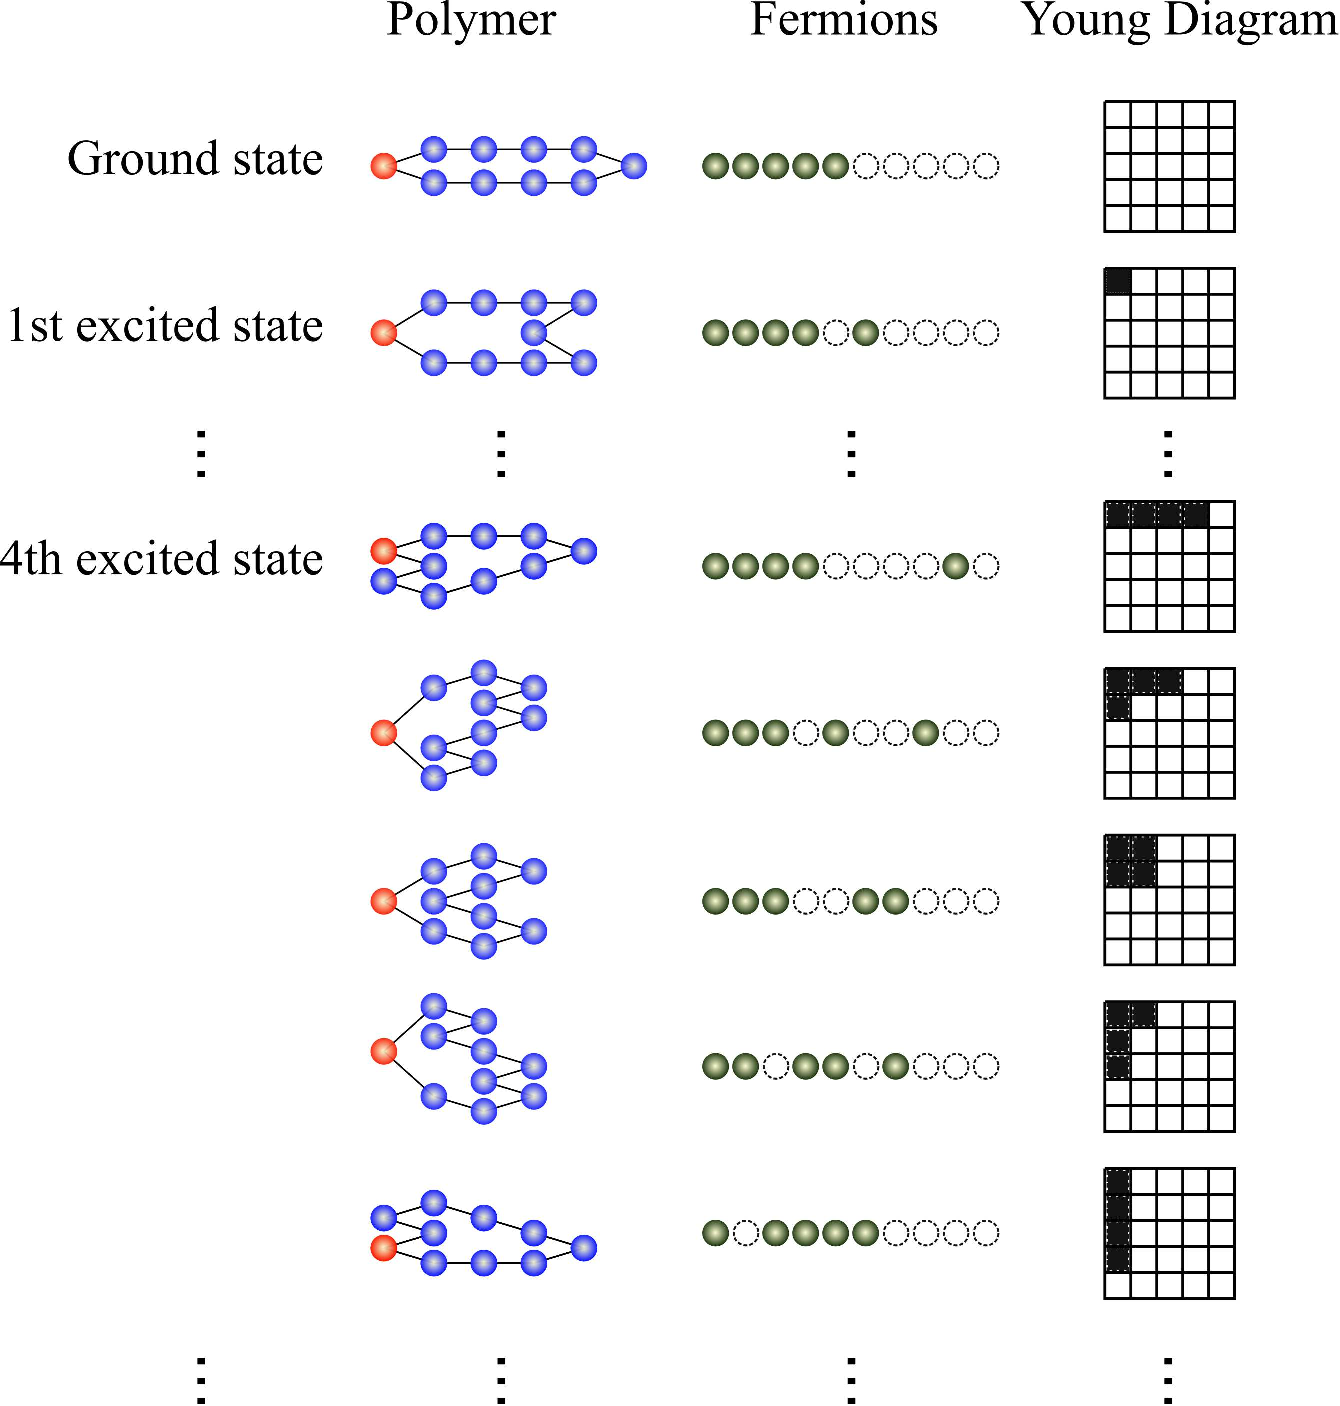
\includegraphics[width=0.45 \textwidth]{schematic}
% \caption{Schematic diagram. (a) Polymer blahblihblah (b) Fermion blahblihblah (c) Young diagram didadi...}
% \label{fig:schematic}
% \end{figure}
%
% \section{Relation to integer partition and number theory} \label{sec:partition} 
% Although the approach detailed in section \label{sec:FD} accurately estimates the mean and variance of equilibrium position of $j^{\rm}$ bead, it is an approximated theory. The random walk is continuous in space and the positions of the beads resides on an lattice. In addition, the distribution of the position of any bead in the random-walk picture is always a Gaussian \cite{klebaner2005introduction}, but in the discrete lattice model it is not: for example, in low temperature, the polymer would be mostly staying in its fully stretched configuration (see Fig.~\ref{fig:schematic}) and the distribution of the positions of the beads are always bounded by the natural length of the rods. 
%
% Analytic solutions are possible in this particular model. We outline the key ideas in the followings, and leave the more detailed and technical analysis in a separate article [XXX]. 
%
% Our idea is to change the basis of the Fermionic system from its microscopic configurations $\l\{Z_0,Z_1,\ldots,Z_{N-1}\r\}$ to the energy of the system. Clearly, the energy can only take values $E_0, E_0+\Delta E, \ldots, E_0 + N^2 \Delta E / 4$; in this picture, the probability space is a one-dimensional lattice with finite support. Without lost of generality, we let the constant energy $E_0=0$ and $\Delta E=1$ by choosing a proper unit. The difficulty of this basis is to determine the degeneracy of the microscopic states which have the same energy $E \in \l\{0,1,\ldots N^2/4\r\}$, sometimes referred to as the ``density of the state'' in statistical mechanics \cite{huang1987statistical} and condensed matter physics \cite{sander2009advanced}. We let the number of microscopic states with energy $E$ to be $g(E)$; once $g(E)$ is known, the partition function of the system can be formally derived in the canonical ensemble picture
% \eq{
% \mathcal{Z}\l(T\r) = \sum_{E=0}^{N^2/4} g(E) \, \exp \l(-\frac{E}{k_B T}\r),
% }{eq:par_func}
% and the equilibrium property of the system can be derived from $\mathcal{Z}$. 
%
% With a little surprise, we discovered that $g(E)$ in this problem is closely related to the problem of integer partition in number theory \cite{andrews1998theory}. The connection can be made by formulating the problem in the following way. We consider to label the micro-state of the system by how many energy unit a Fermion is excited from its ground state. Mathematically, we denote $E_i$ to be the excited energy of the particle with $i^{\rm th}$ highest energy. The total energy of the system is
% \begin{subequations} \label{eq:partition}
% \begin{align}
% E= \sum_{i=1}^{N} E_i,
% \end{align}
% and construction we have a constraint 
% \begin{align}
% N/2 \ge E_1 \ge E_2 \ge \ldots \ge E_{N/2} \ge 0. \label{eq:partition_constraint}
% \end{align}
% \end{subequations}
% Equations \eqref{eq:partition} constitutes a restricted partition of the integer $E$: $g(E)$ is the possible ways to partition an integer $E$ into $N/2$ non-increasing parts \cite{andrews1998theory}.
%
% A very neat way to label the microscopic configuration is to use the Young diagram \cite{andrews1998theory}, showing in the right panel of Fig.~\ref{fig:schematic}. The black box in row $i$ denotes the excited energy $E_i$. With the constraint \eqref{eq:partition_constraint}, each row can have at most $N/2$ black boxes, and the number of black boxes in $(i+1)^{\rm th}$ row cannot exceed the that in $i^{\rm th}$ row.  Then, $g(E)$ is the number of possibility of arrangement of $E$ black boxes onto the $N/2 \times N/2$ ``checkerboard''.
%
% Once the this relation is identified, fruitful results from the number theory \cite{andrews1998theory} can be used to solve our problem. For example, denote  the ways to put $E$ black boxes onto an $K \times L$ checkerboard with non-increasing number of black boxes per row by $\pi \l(K,L,E\r)$. A recursive relation exists \cite{andrews1998theory}
% \eq{
% \pi\l(K,L,E\r) = \pi\l(K,L-1,E\r) + \pi \l(K-1,L, E-L\r),
% }{}
% which allows very efficient computations of the $g(E)=\pi\l(N/2,N/2,E\r)$. In addition, the generating function 
% \eq{
% \Phi \l(q\r) := \sum_{E=0}^{N^2/2} g(E) q^E
% }{}
% is identified to be the Gaussian binomial coefficient
% \eq{
% \Phi \l(q\r) \equiv \l(\begin{array}{c} N \\ N/2 \end{array}\r)_q := \frac{\prod_{j=1}^{N} \l(1-q^j\r)}{\l[\prod_{j=1}^{N/2} \l(1-q^j\r)\r]^2},
% }{}
% which allows us to formulate the partition function of the original polymer problem \eqref{eq:par_func}. 
%
% We finally remark that along this line of analysis, the probability distribution analogous to \eqref{eq:discrete_prob} can also be formulated. Not surprisingly, for a finite (and small $N$), the exact results are different from \eqref{eq:discrete_prob}. Several other physical quantities at equilibrium can be efficiently computed without resorting to Monte Carlo simulation. We will present a more detailed analysis separately [XXX].  
%

\subsection{Brownian bridge}
\subsection{Fermi-Dirac statistics of rod orientations}
\subsection{Fermion integer number partition theory}
\subsection{From rods to a polymer, beauty of Gaussian statistics}

\section{Asymmetric Exclusion Process}
Having shown the equilibrium statistics been solved by mapping from polymer to
particle, we now come to the discussion about the dynamics. It is intuitively to
extend the analogy to nonequilibrium, i.e., the dynamics of pinned polymer
corresponds to particle diffusion in a one dimensional lattice. To illustrate
the equivalence, we firstly define a typical particle hopping model and build
the connection between these two models. 

As shown in the section above, we consider a 1D lattice with $N$ lattice sites and
exact $N/2$ particles. Only simple exclusive interaction between particle is
applied, which means that one lattice site can only occupied by at most one
particle and the order of particles is conserved during the particle hopping
process. Denote the probability of particle hopping to right and left with $p$
and $q$ respectively, we have the following detailed balance during the hopping
\begin{equation}
    p P_{n} = q P_{n+1} \label{eq:db}
\end{equation}
where $P_{n}$ is the probability of configuration before particle hopping to
the right and $P_{n+1}$ is the probability of configuration after hopping. 
In addition, the ratio of of probability should be proportional to a Boltzmann
factor with the energy difference between these two configurations. Eq
\ref{eq:db} can be rewrite as 
\begin{equation}
    q / p = P_{n} / P_{n+1} = \exp{(-\Delta E / k_B T)}  \label{eq:p_divide_q}
\end{equation}

On the other hand, for a specific particle hopping system, the total hopping
rate is determined by the temperature. External force changes nothing but the
ratio $q/p$. Thus we have
\begin{equation}
    p + q = cT \label{eq:p_plus_q}
\end{equation}
where $c$ is a constant. With eq. \ref{eq:p_plus_q} and eq. \ref{eq:p_plus_q}
we can in principle solve $p$ and $q$ uniquely. The key quantity here is
$\Delta E$, which actually connects polymer and particle model. One can learn
from the polymer and particle equivalence that one particle hopping the right
corresponds to the change of two consecutive rods orientation from right-left to
left-right. Thus the energy difference of the two configuration writes
\begin{equation}
    \Delta E = 2F\Delta l
\end{equation}
where $F$ is the strength of external force and $\Delta l $ is the rod length.
Plug into the above equations one obtain
\begin{eqnarray}
    \label{eq:p_and_q}
    p & =  & \frac{cT\exp{(-2F\Delta l / k_B T)}}{1+\exp{(-2F\Delta l / k_B
            T)}} \\
    q & =  & \frac{cT}{1+\exp{(-2F\Delta l / k_B T)}}
\end{eqnarray}
Now we have a well defined particle hopping model equivalent to polymer
dynamics in the bulk, but the boundary condition is still not specified. It
turns out the boundary condition combined with particle number are crucial to
determinate the type of corresponding polymer.


\section{Towards understanding dynamics}

\section{Conclusions}

\begin{acknowledgments}
We would like to acknowledge stimulating discussions with M. Majumdar.\end{acknowledgments}


% \begin{thebibliography}{10}
% \end{thebibliography}

\end{document}
